\documentclass{article}
\usepackage{amsmath}
\usepackage{amssymb}
\usepackage{graphicx}
\usepackage{hyperref}
\usepackage[version=4]{mhchem}


\begin{document}
Point \(E\) is selected on side \(A C\) of triangle \(A B C\) in such a way that \(A E\) : \(E C=3: 4\) and point \(D\) is selected on side \(B C\) so that \(B D: D C=2: 3\). The point of intersection of \(A D\) and \(B E\) is \(F\). Then \(\frac{A F}{F D} \times \frac{B F}{F E}\) is\\
(A) \(\frac{7}{3}\)\\
(B) \(\frac{14}{9}\)\\
(C) \(\frac{35}{12}\)\\
(D) \(\frac{56}{15}\)\\
(E) \(\frac{3}{1}\)\\
\centering
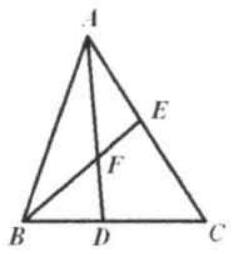
\includegraphics[width=\textwidth]{images/106.jpg}

Solution: (C).\\
Draw \(E G / / B C\) such that \(E G\) meets \(A D\) at \(G\).\\
By similar triangles, \(\frac{G E}{B D}=\frac{G E / D C}{B D / D C}=\frac{A E / A C}{B D / D C}=\frac{3 / 7}{2 / 3}=\frac{9}{14}\).\\
Therefore \(\frac{F G}{D F}=\frac{F E}{B F}=\frac{G E}{B D}=\frac{9}{14}\).\\
We also have \(\frac{D G}{D F}=\frac{23}{14}, \frac{A G}{A D}=\frac{3}{7}\), so \(\frac{G D}{A D}=\frac{4}{7}\)\\
\centering
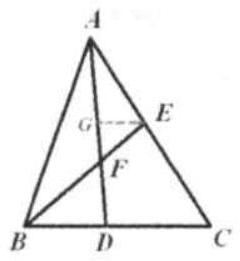
\includegraphics[width=\textwidth]{images/106(1).jpg}\\
\(\Rightarrow G D=\frac{4}{7} A D\).


Thus \(\frac{A D}{D F}=\frac{\frac{7}{4} G D}{D F}=\frac{7}{4} \cdot \frac{23}{14}=\frac{23}{8}\).\\
We also know that \(\frac{A E}{D F}=\frac{15}{8}\).\\
Therefore \(\frac{A F}{F D} \times \frac{B F}{F E}=\frac{15}{8} \times \frac{14}{9}=\frac{35}{12}\).\\

\end{document}
